\begin{figure}[h]
    \centering
    \begin{minipage}[b]{0.4\linewidth}
            \begin{subfigure}[b]{\linewidth}
        \centering
        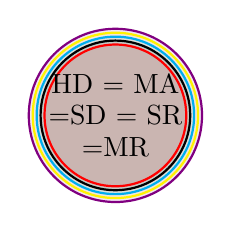
\begin{tikzpicture}
            \draw[thick,violet] (0,0) circle (1.1cm);
            \fill[violet, opacity=0.1] (0,0) circle (1.1cm);
            
            \draw[thick,yellow] (0,0) circle (1.05cm);
            \fill[yellow, opacity=0.1] (0,0) circle (1.05cm);
            
            \draw[thick,cyan] (0,0) circle (1cm);
            \fill[cyan, opacity=0.1] (0,0) circle (1cm); 

            \fill[black, opacity=0.1] (0,0) circle (0.95cm);;
            \draw[thick,black] (0,0) circle (0.95cm);
            
            \draw[thick,red] (0,0) circle (0.9cm);
            \fill[red, opacity=0.1] (0,0) circle (0.9cm);

            \node at (0,0.4) {HD = MA};
            \node at (0,0) {=SD = SR};
            \node at (0,-0.4) {=MR};
        \end{tikzpicture}
    \caption{Safety}
    \end{subfigure}%
    \vfill
    \begin{subfigure}[b]{\linewidth}
        \centering
        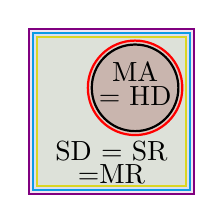
\begin{tikzpicture}
            \draw[thick,cyan] (-1,1) rectangle (1,-1);
            \draw[thick,yellow] (-0.95,0.95) rectangle (0.95,-0.95); % Object 4
            \fill[violet, opacity=0.1] (-1.05,1.05) rectangle (1.05,-1.05);
            \fill[cyan, opacity=0.1] (-1,1) rectangle (1,-1); 
            \fill[yellow, opacity=0.1] (-0.95,0.95) rectangle (0.95,-0.95);
            \draw[thick,violet] (-1.05,1.05) rectangle (1.05,-1.05);

            
            \draw[thick,red] (0.3,0.3) circle (0.6cm);
            \fill[red, opacity=0.1] (0.3,0.3) circle (0.6cm);
            \draw[thick,black] (0.3,0.3) circle (0.55cm);
            \fill[black, opacity=0.1] (0.3,0.3) circle (0.55cm);
            \node at (0,-0.5) {SD = SR};
            \node at (0,-0.8) {=MR};
            \node at (0.3,0.5) {MA};
            \node at (0.3,0.2) {= HD};
        \end{tikzpicture}
    \caption{Reachability, Weak}
    \end{subfigure}%
    \end{minipage}
    \hfill
    \begin{minipage}[b]{0.5\linewidth}
        \begin{subfigure}[b]{\linewidth}
        \centering
        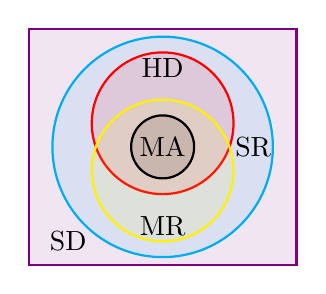
\begin{tikzpicture}
            \draw[thick,violet] (-1.7,1.5) rectangle (1.7,-1.5);
            \fill[violet, opacity=0.1] (-1.7,1.5) rectangle (1.7,-1.5);% Object 1
            \draw[thick,cyan] (0,0) circle (1.4cm);
            \fill[cyan, opacity=0.1] (0,0) circle (1.4cm); % Object 2
            \draw[thick,red] (0,0.3) circle (0.9cm); % Object 3
            \fill[red, opacity=0.1] (0,0.3) circle (0.9cm);
            \draw[thick,yellow] (0,-0.3) circle (0.9cm); % Object 4
            \fill[yellow, opacity=0.1] (0,-0.3) circle (0.9cm);
            \fill[black,opacity=0.1] (0,0) circle (0.4cm);
            \draw[black,thick] (0,0) circle (0.4cm); % Object 5
            \node at (-1.2,-1.2) {SD};
            \node at (1.15,0) {SR};
            \node at (0,1) {HD};
            \node at (0,-1) {MR};
            \node at (0,0) {MA};
        \end{tikzpicture}    \caption{B\"uchi, co-B\"uchi, Parity}
    \end{subfigure}
    \caption{The landscape of automata that admit different resolvers}\label{fig:venndiagrammmmmm}
    \end{minipage}
\end{figure}